%
% Anlagendesign
%
% @version 1.0
% @author dmayer
% @created 29. Dezember 2015

\setchapterpreamble[o]{%
\dictum[--- \textsc{Charles Eames}]{\Gun Design is the appropriate combination of materials in order to solve a problem. \Gob}}
\renewcommand{\chapterheadstartvskip}{\vspace*{2cm}}

\chapter{Anlagendesign}
\label{chap:anlagendesign}

\renewcommand{\chapterheadstartvskip}{\vspace*{-0.5cm}}

Ziel dieses Kapitel ist es, eine Anlage zur Raumtemperaturregelung für den Betrieb mit Modellprädiktiver Regelung zu konzipieren, zu konkretisieren und im letzten Schritt umzusetzen. Dazu werden zunächst die Anforderungen an die Anlage analysiert und weiterhin die Vorgaben und Rahmenbedingungen zur Anlage von Seiten der Hochschule Karlsruhe spezifiziert und ausgeführt. Daraus wird eine Idee abgeleitet, die anschließend zu einem Konzept weiterentwickelt und in ein konkretes Anlagendesign umgesetzt wird. Dabei werden die einzelnen Anlagenteile und deren Funktionsweisen näher beschrieben und auf die realen Einsatzbedingungen ausgelegt. Abschließend wird die Installation und dabei aufgetretenen Besonderheiten der Anlage beschrieben.

Die These, welche es in diesem Kapitel zu belegen gilt, ist, dass sich die beschriebene und umgesetzte Anlage dazu eignet, um die Temperatur innerhalb eines zu regeln. Im nächsten Schritt gilt es zu zeigen, dass sich die Anlage gemeinsam mit dem Einsatz eines in Kapitel \ref{chap:modellbildung} gebildeten Modells, für die Modellprädiktive Regelung eignet.

\section{Analyse der Anforderungen}
\label{sec:anforderungen}

\subsection{Einsatzziele und Rahmenbedingungen}
Um die Anforderungen an eine Anlage zu bestimmen, die sich sich für die Anwendung mit Modellprädiktiver Regelung eignet, wird zunächst der Zweck und die Einsatzziele der Anlage untersucht und definiert. In Kapitel \ref{sec:motivation} wurde bereits darauf hingewiesen, dass es die Vorgabe von Seiten der Hochschule ist, die Einsatzziele in Einklang mit der großen Anlgae zu bringen und komplementär zu wählen. Daher wurden im Dialog mit den Projektverantwortlichen\footnote{In Person von Herrn \textsc{Adrian Bürger} und \textsc{Markus Bohlayer}} für die Forschung im Bereich solarer Anwendungen an der Hochschule Karlsruhe gemeinsam konkrete Einsatzziele der Anlage erarbeitet. Als Ergebnis wurden die folgenden, konkreten Ziele vereinbart:
 
\begin{itemize}
	\item Die Einarbeitung in die Thematiken Modellbildung, Kommunikation von technischen Systemen und Modellprädiktive Regelung soll durch eine praktisches Anwendung unterstützt werden.
	\item Es soll Know-how im Bereich der Kommunikation von technischen Systemen aufgebaut werden, insbesondere im Umgang mit der Software, der Hardware und zahlreichen Schnittstellen.
	\item Die Anlage soll eine hohe Funktionalität, also möglichst wartungsarm, und eine hohe Robustheit gegenüber Fehlern und Beschädigungen besitzen, da bei der Einarbeitung eine erhöhte Wahrscheinlichkeit der Fehlbedienung besteht und Schäden dadurch vermieden werden sollen.
	\item Es soll ein Vergleich verschiedener Regelungsmethodiken beim Einsatz von Modellprädiktiver Regelung ermöglicht werden.
	\item Außerdem soll ein Vergleich von Ergebnissen bei der Variation von Steuerungsparametern sowie beim Einsatz verschiedener Steuerungs- und Regelungsalgorithmen ermöglicht werden.
	\item Des Weiteren soll die Anlage möglichst flexibel ansteuerbar und erweiterbar sein, damit der Grad der Komplexität anpassbar ist und die Anlage um weitere Funktionen oder Features ergänzt werden kann.
	\item Der temperaturerhöhende Effekt der Sonneneinstrahlung auf die Raumtemperatur soll untersucht werden können.
	\item Im Rahmen der Anwendungsforschung soll der Raum zur Temperaturregelung möglichst nahe an der Realität sein, also Störgrößen beinhalten und nicht ungenutzt beziehungsweise leerstehend sein.
\end{itemize}

Zusammenfassend wurde festgehalten, dass die Anlage als Forschungsumgebung für Entwicklungs-, Test- und Anwendungszwecke von verschiedenen Steuerungen und Regelungen dienen soll.

Weiterhin wurden von Seiten der Hochschule Karlsruhe\footnote{In Person von Frau Professor \textsc{Angelika Altmann-Dieses}, Herrn Professor \textsc{Marco Braun} und Herrn \textsc{Adrian Bürger}} Rahmenbedingungen definiert, die im Folgenden zusammengefasst sind:

\begin{itemize}
	\item Der Raum K004a im K Gebäude der Hochschule Karlsruhe wird zur Installation der Anlage und Einrichtung der Forschungsumgebung zur Verfügung gestellt.
	\item Die Installation der Anlage muss mit minimalem baulichem und finanziellem Aufwand zu realisieren sein.
	\item Für die Kommunikation innerhalb der Anlage soll die Modbus Kommunikationstechnologie mit mindestens zwei verschiedenen übertragungsprotokollen genutzt werden.
	\item Die Modellprädiktive Regelung soll mit Hilfe der Plattform JModelica.org erfolgen.
\end{itemize}

\subsection{Definition der Anforderungen}

Diese Einsatzziele und Rahmenbedingungen definieren implizit Anforderungen an eine Anlage, welche im Nachfolgenden explizit ausgeführt werden und aus Gründen der übersichtlichkeit die wichtigsten in Tabelle \ref{tab:anforderungen_umgebung} zusammengefasst sind.


\begin{table}[H]
\centering
\small
\renewcommand{\arraystretch}{1.3}
\begin{tabularx}{1\textwidth}{m{0.35\textwidth}m{0.58\textwidth}}

\toprule

\textbf{Einsatzziele \&} & \multirow{2}{\hsize}{\textbf{Anforderungen}} \\ 
\textbf{Rahmenbedingungen} & \\

\cmidrule[0.5pt](r{0.25em}){1-1} 
\cmidrule[0.5pt](l{0.25em}){2-2}

Raum K004a als Umgebung  & \multirow{3}{\hsize}{
\begin{minipage}[t]{0.57\textwidth}
\begin{itemize}[itemsep=0pt,topsep=0pt,leftmargin=5mm]
	\item Die Anpassung der Anlage an K004a.
	\item Die Nutzung bestehender Heizkörper anstatt einer Klimatisierung des Raumes. 
	\item Die Beschränkung auf eine minimale Funktionalität und Anzahl der einzelnen Komponenten. 
\end{itemize}
\end{minipage}
}
 \\
	
\cmidrule[0.1pt](lr{2em}){1-1} 
Minimaler baulicher Aufwand & \\

\cmidrule[0.1pt](lr{2em}){1-1} 
Minimaler finanzieller \newline Aufwand &\\ 



\cmidrule[0.5pt](r{0.25em}){1-1} 
\cmidrule[0.5pt](l{0.25em}){2-2}

\addlinespace[4mm] Modellprädiktive Regelung mit JModelica.org und CasADi \newline & \multirow{3}{\hsize}{
\begin{minipage}[t]{0.57\textwidth}
\begin{itemize}[itemsep=0pt,topsep=0pt,leftmargin=5mm]
\item Die Modellbildung erfolgt in Modelica.
\item Die Ansteuerung und Kommunikation innerhalb der Anlage soll in Python stattfinden.
\item Die Kommunikation der Anlage erfolgt gemäß den Modbus~RTU und TCP Protokollspezifikationen.
\item über Modbus~TCP soll die Ansteuerung der Anlage innerhalb des gesamten lokalen Netzwerks möglich sein.
\end{itemize}
\end{minipage}
}  \\

\cmidrule[0.1pt](lr{2em}){1-1}
\addlinespace[4mm] Einsatz der Modbus \newline Kommunikationstechnologie \newline 	& 		\\

\cmidrule[0.1pt](lr{2em}){1-1}
\addlinespace[4mm] Flexible Ansteuerung der Anlage \newline & \\

\cmidrule[0.5pt](r{0.25em}){1-1} 
\cmidrule[0.5pt](l{0.25em}){2-2}

Einarbeitung in die Thematiken:
\begin{minipage}[t]{0.34\textwidth}
\begin{itemize}[itemsep=0pt,topsep=0pt,leftmargin=4mm]
	\item Modellbildung,
	\item Kommunikation technischer \newline Systeme,
	\item und Modellprädiktive \newline Regelung.
\end{itemize}
\end{minipage}
 	& \multirow{2}{\hsize}{
\begin{minipage}[t]{0.57\textwidth}
\begin{itemize}[itemsep=0pt,topsep=0pt,leftmargin=5mm]
	\item Komplexität ist notwendig, darf jedoch nicht zu hoch sein.
	\item Es sind möglichst wenige thematische überschneidungen erwünscht, daher wird eine klare Struktur mit möglichst scharfer Trennung benötigt.
\end{itemize}
\end{minipage}
}  \\

\cmidrule[0.1pt](lr{2em}){1-1} 

Know-how für Kommunikation \newline technischer Systeme 	&		\\

\cmidrule[0.5pt](r{0.25em}){1-1} 
\cmidrule[0.5pt](l{0.25em}){2-2}

Vergleich von Ergebnissen durch:
\begin{minipage}[t]{0.34\textwidth}
\begin{itemize}[itemsep=0pt,topsep=1pt,leftmargin=4mm]
	\item die Variation von \newline Steuerungsparametern,
	\item den Einsatz verschiedener \newline Regelungsmethodiken,
	\item und den Einsatz \newline verschiedener Algorithmen.
\end{itemize}
\end{minipage}

& \multirow{3}{\hsize}{
\begin{minipage}[t]{0.57\textwidth}
\begin{itemize}[itemsep=0pt,topsep=0pt,leftmargin=5mm]
\item Die Reaktion des Systems muss schnell sowie günstig und einfach zu erfassen sein.
\item Der Einsatz von robusten und einfachen Bauteile.
\item Nutzung eines wartungsarmen Systems.
\item Eine einfache, modulare Erweiterbarkeit des Systems für weitere Schritte muss gegeben sein.
\end{itemize}
\end{minipage}
}  \\

\cmidrule[0.1pt](lr{2em}){1-1} 

Hohe Funktionalität und \newline Robustheit & \\

\cmidrule[0.1pt](lr{2em}){1-1} 

Erweiterbarkeit der Anlage
 &  \\

\bottomrule
\end{tabularx}
\caption{Umsetzung der Ziele in Anforderungen der Anlage}
\label{tab:anforderungen_umgebung}
\end{table}

Die grundlegendste Anforderung an die Planung, ist die Anpassung an die Lage und die Gegebenheiten des Raumes K004a, welche in \ref{fig:skizzek004a} skizziert sind. Der Raum befindet auf dem Campus der Hochschule Karlsruhe, an der südwestlichen Ecke des K Gebäudes im Erdgeschoss. Die südliche und westliche Wand teilt sich der Raum mit der Außenumgebung und wird im Folgenden als Außenwand bezeichnet. Die östliche und nördliche Wand sowie die Decke und der Boden des Raumes grenzen an andere Räume im K Gebäude. Außerdem ist in der südlichen Außenwand eine Fensterfront mit Jalousien zur Verschattung eingebaut und direkt darunter ein Heizkörper installiert.

\begin{figure}
\centering
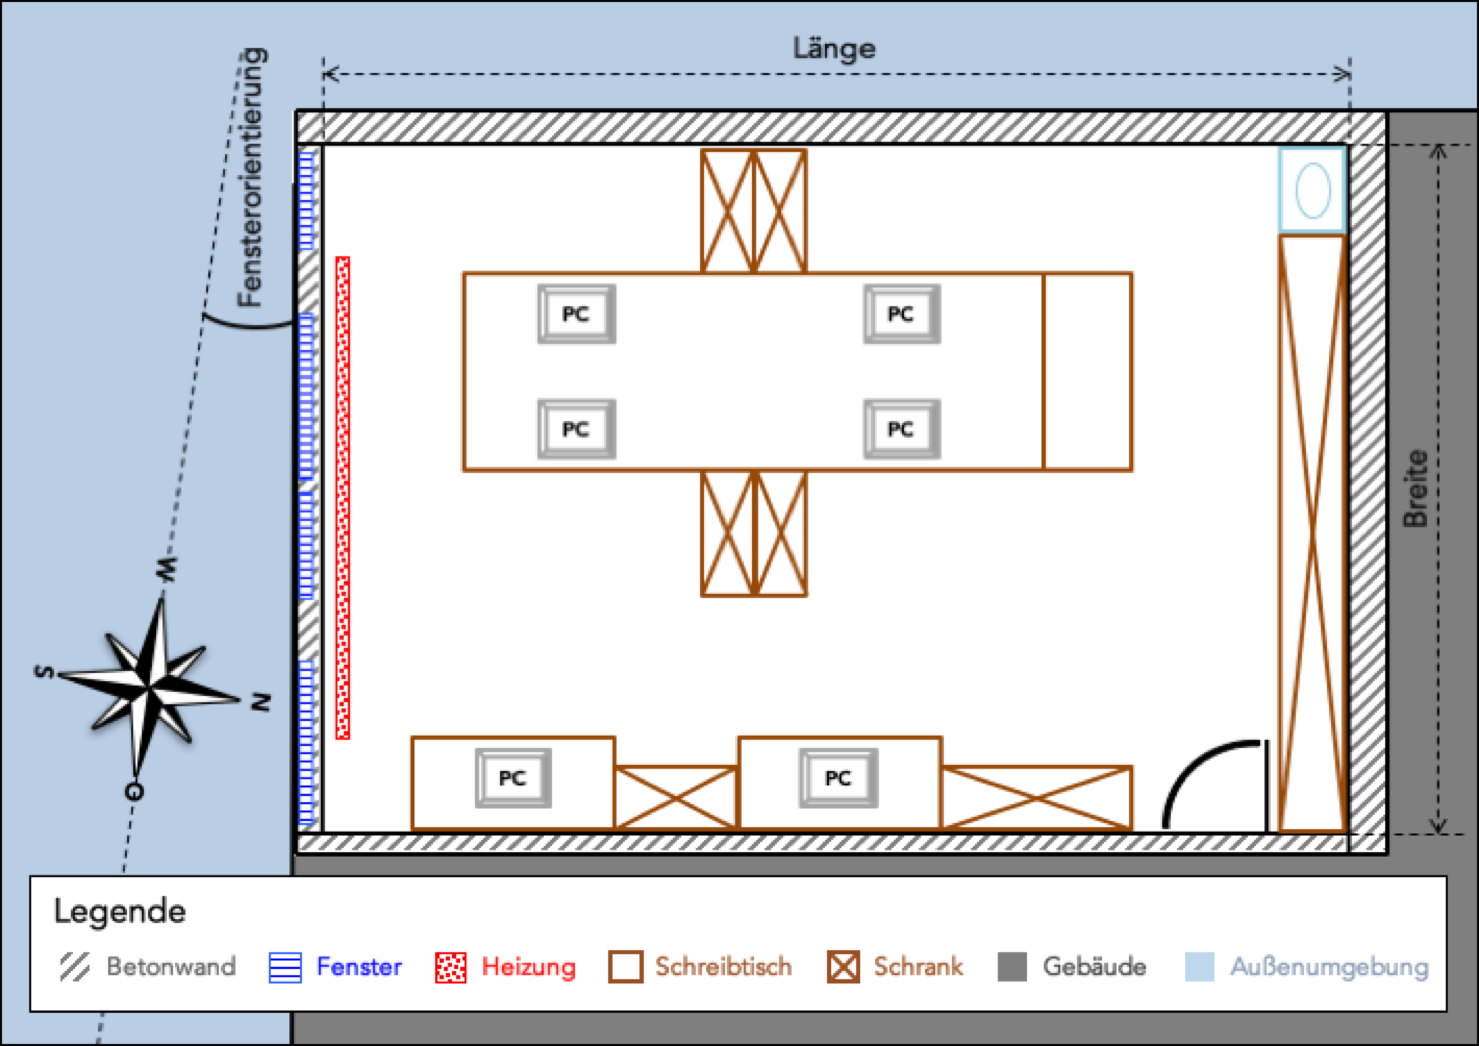
\includegraphics[width=\textwidth]{abbildungen/20160102_k004a}
\caption[Raumskizze K004A vom K Gebäude der Hochschule Karlsruhe -- Technik und Wirtschaft]{Raumskizze K004A vom K Gebäude der Hochschule Karlsruhe -- Technik und Wirtschaft}
\label{fig:skizzek004a}
\end{figure}

Durch die Raumwahl werden bereits zwei wichtige Anforderungen erfüllt, denn durch die Fensterfront kann der Einfluss der Sonneneinstrahlung auf die Raumtemperatur untersucht werden und der bestehende Heizkörper kann in die Anlage integriert werden, um einen minimalen baulichen Aufwand sicherzustellen. Damit wird zunächst eine Klimatisierung zur Temperaturregelung des Raumes ausgeschlossen, weil diese mit einem erheblichen finanziellen und baulichen Aufwand verbunden ist. Um der Forderung nach einer Erweiterbarkeit nachzukommen, wird jedoch die Möglichkeit der Nachrüstung einer Klimatisierung und der Ansteuerung der Jalousien bei der Planung explizit berücksichtigt.

Durch die Nutzung des Raumes als Büro für wissenschaftliche Mitarbeiter befinden sich in K004a sechs Computerarbeitsplätze sowie das typische Büro-Mobiliar, wie in \ref{fig:skizzek004a} abgebildet. Damit wird auch die Anforderung einer anwendungsnahen Umgebung erfüllt und durch die Menschen und Rechner sind verschiedene Störgrößen zu berücksichtigen.

Eine weitere, sehr einschränkende Vorgabe ist es, dass die Modellprädiktive Regelung unter Zuhilfenahme der Plattform \textsc{JModelica.org} erfolgen soll. \textsc{JModelica.org} ist eine kostenlose Open-Source Plattform	 zur Analyse, Simulation und Optimierung von komplexen, dynamischen Systemen, die auf der Modellierungssprache Modelica basiert. Aufbauend auf den mathematischen Modellen physikalischer Systeme in Modelica, lassen sich, dank der Unterstützung der Spracherweiterung Optimica, Optimierungsprobleme durch einfache Konstrukte das Optimierungsintervall, die Kostenfunktion und die Nebenbedingungen einfach formulieren. JModelica.org wird über eine Python Nutzerschnittstelle genutzt und besitzt eine eigene Klasse für die Modellprädiktive Regelung, auch wenn diese bisher noch experimenteller Art ist \cite[S.~1f.]{jmod15}.
Der Compiler kann die Modelle und Optimierungsprobleme in verschiedene Formate übersetzen. Zum einen in direkt ausführbaren C Code, der die Modellgleichungen und Optimierungsparameter enthält, und ein XML Code, der die Meta-Daten des Modells enthält. Zum anderen kann das Modell aber auch in ein \textit{OptimizationProblem} Objekt transferiert werden, welches eine symbolische Repräsentation des Optimierungsproblems ist \cite[S.~12ff.]{jmod15}.

Die \textit{OptimizationProblem} Objekte können anschließend direkt mit den Optimierungswerkzeugen von \textsc{CasADi} bearbeitet und damit zur Lösung des Optimierungsproblems eingesetzt werden. \textsc{CasADi} ist ein Open-Source Softwaretool, das einzelne Bausteine für die numerische Optimierung im Allgemeinen und für die Optimalsteuerung im Speziellen zur Verfügung stellt. Es eignet sich besonders für die gradientenbasierte, numerische Optimierung von nichtlinearen Problemen, aufgrund seiner effizienten Ableitungserzeugung durch die Algorithmische Differentiation und und der Möglichkeit zur Integration von gewöhnlichen Differenzialgleichungen und differential-algebraischer Gleichungen. Die Interaktion mit dem Nutzer soll aus Stabilitätsgründen über die Python Schnittstelle erfolgen \cite[S.~5f.]{casadi}.
Daraus resultieren weitere Anforderungen an das Modell, welche vor Beginn der Modellbildung im Kapitel \ref{chap:modellbildung} erörtert werden.

%Until here fine

Weil die vorgegebene Softwareplattform zur Modellprädiktiven Regelung und deren Komponenten eine allesamt eine Schnittstelle für Python besitzen, soll die Ansteuerung und Kommunikation der gesamten Anlage in Python erfolgen. Python eignet sich hervorragend für diese Aufgabe, da es frei erhältlich und modular aufgebaut ist. Durch die Open-Source Lizenzierung ist es frei nutzbar und bietet sowohl durch die Standardbibliothek als auch durch eine Vielzahl an nutzerentwickelten Bibliotheken, die auch als Pakete bezeichnet werden, unzählige Anwendungsmöglichkeiten, zum Beispiel das pysolar Paket, das im Rahmen der Modellbildung eine Umrechnung der gemessenen Solarstrahlung in die wirkende am Fenster ermöglicht \cite[S.~2f.]{python}.

Der Vorgabe der Modbus Kommunikationsprotokolle für die Kommunikation ist von ebenfalls von großer Relevanz, da die komplementäre Forschungsanlage zur solaren Klimatisierung dasselbe Kommunikationsprotokoll unterstützt und durch die gewonnenen Erkenntnisse eine beschleunigte Inbetriebnahme erfolgen kann. Um das Know-how breit zu fächern, sollen die beiden Modbus RTU und Modbus TCP Protokolle Anwendung finden. Außerdem soll das Kommunikationsnetzwerk aus mehreren Subnetzwerken aufgebaut sein, die durch verschiedene elektrische und mechanische Schnittstellen implementiert werden. Für die Kommunikation über Modbus werden in den Python Paketen pymodbus, minimalmodbus und modbus-tk bereits Bausteine zur Verfügung gestellt.

Die Anlage sollte möglichst wenig Komplexität aufweisen, damit die Einarbeitung in die einzelnen Themengebiete Modellbildung, Kommunikation von technischen Systemen und Modellprädiktive Regelung vereinfacht wird. Dies soll durch eine klare Abgrenzung der verschiedenen Anlagenteile und deren Funktionen sowie durch die Strukturierung und den Aufbau der Anlage erreicht werden.Im Gegensatz dazu steht die Forderung nach dem Aufbau von Know-how auf dem Gebiet der Kommunikation technischer Systeme. Deshalb muss ein Kompromiss zwischen Verständlichkeit und Komplexität gefunden werden, um beiden Anforderungen gerecht zu werden. Dieser besteht darin, dass die Kommunikation nur über Modbus stattfindet, jedoch unter Nutzung von verschiedenen Hard- und Software-Schnittstellen, um einen gewissen Grad an Komplexität zu erreichen. Zudem können dadurch bereits Erfahrungen gesammelt werden, die für die Inbetriebnahme der solaren Klimatisierungsanlage sehr nützlich sind. 

Um das Vergleichen von Ergebnissen zu ermöglichen, soll das System auf eine änderung der Steuergrößen schnell\footnote{Im Kontrast zu den langsamen Reaktionen der solaren Klimatisierungsanlage, welche im oberen Minutenbereich liegen, bedeutet schnell in diesem Kontext im unteren Minutenbereich.} reagieren und die Reaktionen sollen möglichst einfach messbar sein. 
Konkret lässt sich daraus ableiten, dass die Aktorik auf Steuersignale möglichst ohne zeitliche Verzögerung agieren sowie die gesamte Anlage einen möglichst direkten Einfluss auf die Raumtemperatur haben soll. 
Die Messung der Raumtemperatur kann durch einfache Temperatursensoren erfolgen die ohne großen technischen und monetären Aufwand auskommen und damit die Anforderung erfüllen.

Es soll außerdem eine hohe Funktionalität erreicht werden, um die wissenschaftliche Arbeit -- durch den Ausschluss von Fehlerquellen außerhalb der Forschung -- zu erleichtern. 
Zusätzlich ist eine Robustheit gegenüber Bedienungsfehlern und Beschädigungen erforderlich, da durch den Test- und Entwicklungsauftrag der Anlage hierzu eine erhöhte Gefahr besteht. Dies lässt sich durch wartungsarme, robuste und einfache Bauteile sowie den Aufbau der Anlage berücksichtigen, was wiederum im Einklang mit der Forderung nach einer minimalen finanziellen Belastung steht.

Wie an passender Stelle bereits erwähnt, stellt Python Schnittstellen und Funktionalitäten für die Aufgaben der Anlage zur Verfügung. Darüberhinaus bietet sich Python, durch die weitgehende Unabhängigkeit vom Betriebssystem, als zentrales Steuerungstool an, um den Controller in einem nächsten Schritt durch einen vergleichsweise günstigen Einplatinenrechner zu realisieren, wie zum Beispiel ein Raspberry Pi. Daher basiert die folgende Planung und Auslegung der Anlage auf einer zentralen Steuerung in Python.

\section{Ziel und die Idee der Anlage}


\subsection{Aufgabe der Anlage}
Das Ziel ist es, die Temperatur innerhalb eines Raumes mit Hilfe eines technischen Systems zu regeln, welches den zuvor ausgeführten Anforderungen genügt.

Dazu gilt es zunächst, die Raumtemperatur über einfache Raumtemperaturfühler zu erfassen. Ist die Raumtemperatur bekannt so soll diese mit Hilfe eines Heizkörpers beeinflusst werden, damit sie einer vorgegebener Temperaturkurve folgen kann. 

Die Heizleistung wiederum hängt von weiteren Eigenschaften des Heizkörpers ab und wird über das Einlassventil gesteuert. Sie wird von einem Wärmemengenzähler gemessen und indirekt über den Massenstrom und die Temperaturen des Heizwassers am Ein- und Auslass bestimmt. Dazu werden ein Durchflusssensor sowie zwei Temperatursensoren an den jeweiligen Enden des Heizkörpers eingesetzt. Um die Heizleistung zu steuern, muss also der Massenstrom gemessen und gesteuert werden sowie beide Temperaturen am Heizkörper bekannt sein. über das Ventil kann der Massenstrom mit Hilfe eines Stellantriebs eingestellt werden. Zusammen mit der Temperatur am Einlass und den Eigenschaften des Heizkörpers, lässt sich die Temperatur am Auslass und damit die aktuelle Heizleistung bestimmen. Dadurch wird eine gezielte Beeinflussung der Raumtemperatur ermöglicht.

Nachdem die Raumtemperatur bekannt ist und eine Möglichkeit für deren Manipulation besteht, wird weiterhin eine intelligentee Steuerung benötigt. Dieser soll den Heizkörper möglichst ressourcenschonend einsetzen, um das Ziel der Temperaturregelung zu erreichen.

\subsection{Idee der Anlage}

Diese umfassende Aufgabe wird von einer Anlage übernommen, die sich dazu grob in drei Teile gliedern lässt. Den größten Umfang besitzt die Sensorik, die zur quantitativen Erfassung der Zuständsgrößen dient. Die aktive Beeinflussung dieser Größen erfolgt durch die Aktorik. Die Regelungsaufgabe wird von einem Controller durch seine interne Logik und der Koordination des Zusammenspiels zwischen Sensorik und Aktorik gelöst.

Um den Anforderungen gerecht zu werden, muss der logische Controller als zentrale Komponente der Anlage Python unterstützen und die gesamten Steuerungs- und Kommunikationsaufgaben übernehmen. Weiterhin müssen im Rahmen der Modellprädiktiven Regelung in regelmäßigen Zeitabständen wiederholt Optimalsteuerungsprobleme gelöst werden, weshalb eine ausreichende große Rechenkapazität benötigt wird. Um diesen Aufgaben übernehmen zu können und um keinen zusätzlichen finanziellen Aufwand zu generieren, wird zunächst ein freier Rechner der Hochschule Karlsruhe als Controller genutzt.  

Wie bereits beschrieben hat die Sensorik den größten Umfang, da sie neben der Raumtemperatur auch den Massenstrom und die Temperaturen am Heizkörper erfasst. Die Temperatur innerhalb des Raumes wird durch mehrere Sensoren erfasst, um die unterstellte Homogenität zu überprüfen und für die Modellberechnungen herzustellen. Für die Erfassung der Heizleistung wird ein Wärmemengenzähler eingesetzt, der wiederum aus einem Rechenwerk, zwei weiteren Temperatursensoren und einem Durchflusssensor aufgebaut ist. Für die Modellprädiktive Regelung werden die einzelnen Werte aller Sensoren benötigt, weshalb das Rechenwerk einen Zugriff darauf ermöglichen muss.

Die Aktorik umfasst lediglich die Ansteuerung des Heizungsventils. Wie zuvor bereits erwähnt wird dazu ein Stellantrieb genutzt, um das Ventil stufenlos zu öffnen und zu Schließen und damit den Massenstrom bis hin zu einem Maximalwert zu steuern. 

Eine Prinzipskizze dieser Idee ist in \ref{fig:konzept} graphisch dargestellt.

\begin{figure}
\centering
\includegraphics[width=\textwidth]{abbildungen/20160318_Konzept}
\caption{Prinzipskizze eines technischen Systems zur Raumtemperaturregelung des Raumes K004b}
\label{fig:konzept}
\end{figure}

\section{Konzept und Planung}
 
Das folgende Konzept erfüllt die in Abschnitt  \ref{sec:anforderungen} definierten Anforderungen und konkretisiert die zuvor geschilderte Idee. Zunächst das Netzwerk, dann xxx bis xxx

\subsection{Netzwerkarchitektur}

Der Rechner stellt das Zentrum der Anlage dar, deshalb werden darauf aufbauend die Kommunikationsleitungen und der Aufbau des Netzwerk geplant. Die Kommunikation erfolgt gemäß den Spezifikationen der beiden Modbus Protokolle RTU und TCP, deren Besonderheiten im Abschnitt \ref{sub:modbus} beschrieben wurden. Da der Rechner standardmäßig mit einem Ethernet-Netzwerkanschluss ausgestattet ist, wird der Rechner über ein Netzwerkkabel mit dem ersten Subnetzwerk verbunden. Das erste Netzwerk ist also ein lokales Netzwerk, das gemäß dem Ethernet/IP Protokoll ausgeführt ist und damit die Kommunikation über das Modbus TCP Protokoll ermöglicht.

Das zweite Subnetz ist ein serielles RS 485 Netzwerk und erlaubt somit den Einsatz des Modbus RTU Protokolls. Die beiden Netzwerke werden durch ein Gateway miteinander verbunden, welches die Übersetzung der Kommunikation in beiderlei Richtungen übernimmt. Die Übersetzung beinhaltet im Detail das Umwandeln der elektrischen Signale und der verschiedenen Modbus Telegrammformate ineinander.

Das eingesetzte \textsc{EX9132C-2-MTCP} Gateway von \textsc{ExpertDAQ} bietet hierzu eine einfache und kostengünstige Möglichkeit, um von einem Modbus TCP/IP Clienten aus mit Modbus RTU Servern zu kommunizieren. Es verfügt über zwei serielle Ports verfügt, jeweils ein EIA-232 und ein EIA 485 Port. Die genauen Spezifikationen können dem Datenblatt im Anhang \ref{att:ex9132} entnommen werden.

Im dritten Subnetz wird über analoge Spannungssignale und Stromsignale kommuniziert, welche von einem Signalwandler erzeugt werden. Der Signalwandler wiederum ist kein Gateway, da die Spannungssignale nicht implizit übersetzt, sondern explizit durch Modbus RTU Befehlstelegramme festgelegt werden. Eine graphische Zusammenfassung der Netzwerkarchitektur ist in \ref{fig:netzwerk} abgebildet.

\begin{figure}
\centering
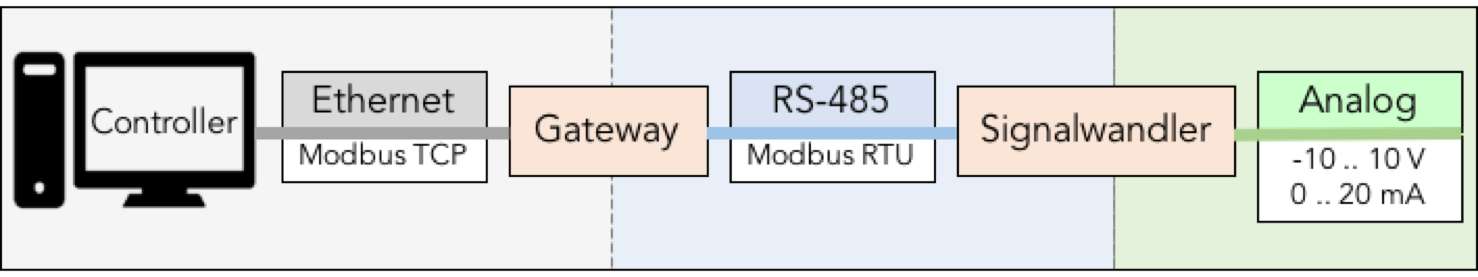
\includegraphics[width=\textwidth]{abbildungen/20160324_netzwerk}
\caption{Aufbau des Netzwerks}
\label{fig:netzwerk}
\end{figure}

\subsection{Erfassung der Raumtemperatur}

Die Raumtemperatur kann einfach und günstig mit Raumtemperaturfühlern gemessen werden. Zudem soll der gemessene Wert über eine der beiden Modbus Schnittstellen dem Controller zur Verfügung gestellt werden. Innerhalb der Anlage kommen zwei \textsc{THERMASGARD RTM1-Modbus} Raumtemperaturfühler ohne Display von \textsc{S+S Regeltechnik} zum Einsatz, weil sich diese durch weitere Eigenschaften, wie zum Beispiel der Kalibrierfähigkeit, auszeichnen. Die detaillierten Funktionen und Daten können dem Datenblatt im Anhang \ref{att:rtm1} entnommen werden.

Ursprünglich sollten die beiden Temperatursensoren auf einer mittig gedachten Achse im Raum in nord-südlicher Richtung platziert werden, jeweils am Ende des mittigen Schreibtischs. Jedoch wurden während der Installation der Anlage noch vier weitere Temperatursensoren zusammen mit einem Messumformer von Seiten der Hochschule Karlsruhe zur Verfügung gestellt. 
Bei den Sensoren handelt es sich um vier PT1000 Temperatursensoren die über den \textsc{Webthermograph 8x} von \textsc{WuT} die Messwerte zur Verfügung stellen. Der Webthermograph besitzt keine Modbus Schnittstelle, jedoch kann er über ein Netzwerkkabel in das Ethernet Netzwerk integriert werden und unter Verwendung des HTTP Protokolls vom Controller ausgelesen werden.
Um die Messwerte mit dem Controller auszulesen, bietet sich das Python Paket \textit{httplib} an, welches das HTTP Protokoll implementiert und einfache Funktionen zur Verfügung stellt. 
Die Anordnung der Temperatursensoren wurde daher angepasst, sodass jeweils drei Sensoren an gegenüberliegenden Wänden angeordnet sind. Die Sensoren wurden entlang der westlichen Außenwand und der östlichen Innenwand gleichmäßig verteilt und auf einer Höhe von 2~m installiert. Die Identifizierung der Sensoren erfolgt über ID´s, die zusammen mit der Anordnung in \ref{fig:raumtempsensors} visualisiert sind.

\begin{figure}
\centering
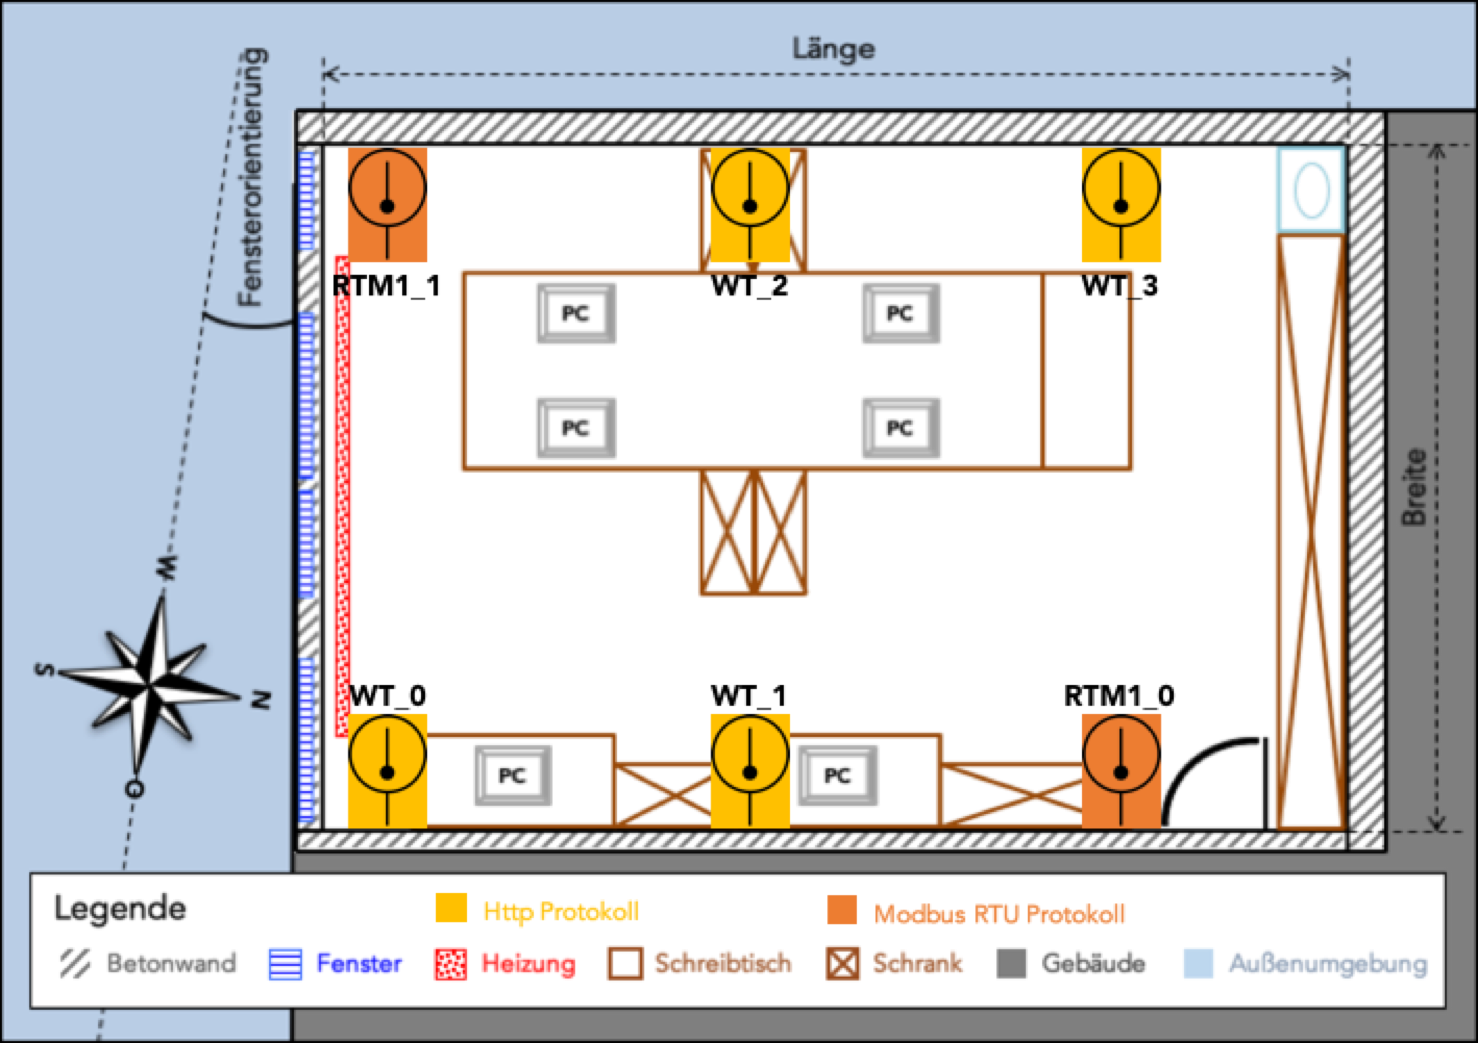
\includegraphics[width=\textwidth]{abbildungen/20160324_sensors}
\caption{Verteilung der Raumtemperaturfühler}
\label{fig:raumtempsensors}
\end{figure}

\subsection{Steuerung des Heizkörpers}

Um die Heizung mit den benötigten Sensoren auszustatten, bietet sich wie bereits erwähnt ein Wärmemengenzähler an. Die Temperaturmessung am Ein- und Auslass der Heizung gestaltet sich jedoch etwas aufwendiger als zuvor. Dazu werden Tauchhülsen im Vor- und Rücklauf des Heizkörpers benötigt, welche vom Heizwasser direkt umflossen werden. Die Tauchhülsen bedingen geringe bauliche Änderungen und können beispielsweise in einen Kugelhahn eingeschraubt werden. Sie sind jeweils mit einem Temperaturfühler bestückt und ermöglichen dadurch die Messung der Heizwassertemperatur. Der Einbau des Durchflusssensors erfordert ebenfalls bauliche Maßnahmen. Dazu wird entweder im Vor- oder Rücklauf, je nach Spezifikation Herstellers, ein Stück Rohrleitung entfernt und durch den Durchflusssensor ersetzt. Dieser kann beim Einbau entweder fest integriert oder durch eine Anschlussverschraubung beziehungsweise einen Flanschanschluss einfach demontierbar eingebaut werden.

In der Anlage kommt der Wärmemengenzähler \textsc{MULTICAL 602} von \textsc{Kamstrup} zum Einsatz, da er neben einem geforderten Modbus Kommunikationsmodul weitere besondere Eigenschaften mit sich bringt. Die Temperaturen werden von zwei PT500 Sensoren erfasst und der Durchfluss von einem \textsc{ULTRAFLOW 54} Ultraschallsensor gemessen. Die gemessenen und  berechneten Werte der Heizungsleistung lassen sich einfach einzeln durch das Rechenwerk einfach auslesen.
Der \textsc{MULTICAL 602} ist zum einen kostengünstig und umfasst alle benötigten Sensoren, die außerdem bereits präzise aufeinander abgestimmt sind. Zum anderen ist er wartungsfrei, da der Durchfluss über kontaktlose Ultraschallmessungen bestimmt wird, indem er die Laufzeitdifferenz zwischen wechselseitig gesendeten und empfangenen Signalen zweier integrierter Ultraschallsensoren auswertet. Zudem ist der Durchflusssensor \textsc{ULTRAFLOW 54} bereits mit einer Tauchhülse ausgestattet, sodass lediglich eine weitere Tauchhülse montiert werden muss.


Die Steuerung des Durchflusses im Heizkörper erfolgt über das Heizungsventil, welches mit Hilfe eines Stellantriebs geöffnet und geschlossen wird. Dieser kann von einem Elektromotor angetrieben werden, der sich durch eine schnelle Reaktion aber hohe Anschaffungskosten  auszeichnet. Alternativ kann ein thermoelektrisches Element als Antrieb genutzt werden, welches sich durch geringe Anschaffungskosten auszeichnet jedoch eine langsamere Reaktionszeit besitzt. Die Ansteuerung des Stellantriebs erfolgt üblicherweise unabhängig von der Ausführung durch ein digitales oder analoges Spannungs- oder Stromsignal.

Um dem Controller die Steuerung zu ermöglichen, wird ein Signalwandler eingesetzt, der Modbustelegramme in elektrische Signale umwandeln kann. Dazu wird innerhalb der Anlage das \textit{EX9024-M} Modul von \textsc{ExpertDAQ} eingesetzt, welches sich leicht in ein serielles RS485-Netzwerk einbinden lässt. Das Modul ist Modbus RTU-fähig und besitzt vier analoge Ausgänge die verschiedene Spannungs und Strombereiche ausgeben können. Da für den Stellantrieb lediglich ein Ausgang genutzt wird, besteht explizit die Möglichkeit einer einfachen Erweiterung der Anlage um 3 weitere, analoge Komponenten, beispielsweise einem Schalter zur Bedienung  der Jalousien.

Der thermoelektrische Stellantrieb \textit{ABNM-LIN} von \textit{Danfoss} wird zur stufenlosen Betätigung des Heizkörperventils eingesetzt. Die Ansteuerung erfolgt über ein analoges 0-10~V Signal, welches innerhalb der Anlage vom EX9024-M bereitgestellt wird. Der Stellantrieb wandelt das angelegte Signal in einen proportionalen, linearen Stellweg um und steuert damit den Durchfluss im Heizkörper.

Das beschriebene Konzept zeichnet sich dadurch aus, dass es eine kostengünstige Umsetzung erlaubt und eine größtmögliche Kompabilität der Anlageteile und Bauteile sicherstellt. Die explizit Forderung nach der Erweiterbarkeit wird explizit durch die offene Architektur und die eingesetzten Komponenten ebenfalls berückscihtigt, sodass langfristig die Möglichkeit besteht die Raumtemperatur beispielsweise unter Zuhilfenahme einer Raumklimatisierung und der Ansteuerung der Jalousien ganzjährig zu regeln zu können.

\section{Installation und Inbetriebnahme}

Eine Übersicht über den Aufbau der Anlage findet sich in Abbildung REFXXXXX. Die ionstallation gliedert sich ein zwei Bereiche, zunöchst der Hardware Installation, die die  Montage der einzelnen Kompononten, deren Stromversorgung und die Verkabelung im Netzwerk umfasst.
Der zweite Teil beschäftigt sich mit der Inbetriebnhame der Anlage durch die Softwareseitige Ansteuerung und Benutzung der Anlage.


\subsection{Hardware}

Der Aufbau des Netzwerks wurde bereits in \ref{fig:netzwerk} dargestellt. Als Ethernet-Netzwerk wird das lokale Netzwerk der Hochschule Karlsruhe genutzt. Dadurch ist die flexible Ansteuerung der Anlage innerhalb des gesamten lokalen Netzwerks und über eine VPN-Verbindung auch außerhalb vom Campus möglich, auch wenn dadurch zusätzlich ein Passwortschutz erforderlich wird. Der Rechner ist bereits im Netzwerk integriert, sodass ledglich das Gateway beim IZ der Hochschule Karlsruhe registriert werden musste, um eine IP Adressierung gemäß dem Ethernet/IP Protokoll zu erhalten.
Für den Webthermographen wurde dasselbe Procedere durchlaufen, um diesen in die Anlage zu integrieren.

Der Schaltplan des seriellen RS-485 Netzwerk wird in \ref{fig:schaltplan} dargestellt. Zur Verkabelung de Netzwerks wird eine Busleitung von LappKabel eingesetzt, welche zwei jeweils paarweise verdrillte Leitungspaare
besitzt die durch ein Kupfergeflecht von Störungen abgeschirmt sind. Das Datenblatt der Busleitung ist in nahang XXXX zu finden.
Gemäß der Spezifuikationen im Modbus seriell Protokoll ZITAT erfolgt die Verkabelung der D0 Leitung die braubne sowie der D1 Leitung die gelbe Ader zugewiesen. Die GNC Common wird über die weißgraue Ader verdrahtet. Das grüne Kabel kann für die gemeinsame Stromversogung der Komponenten genutzt werden, was im Rahmen dieser anlage durch die verschiedenen benötigten Spannungen nicht genutzt wurde. Daher hat jede Komponente ihre eigene Stromversorgung durch jeweils ein eigenes Netzteil gemäß dem Schaltplan. 

Die Kabel wurden gemäß der Übersicht in REFFFFXXXX verlegt und mit den Bauteilen gemäß dem Schaltplan in ref{fig:schaltplan} verbunden. Die kurzen Stichleitungen wurden über flexibel einsetzbare sowie wiederverwendbare Hebelklemmen an die lange Busleitung angeschlossen.


\begin{figure}
\centering
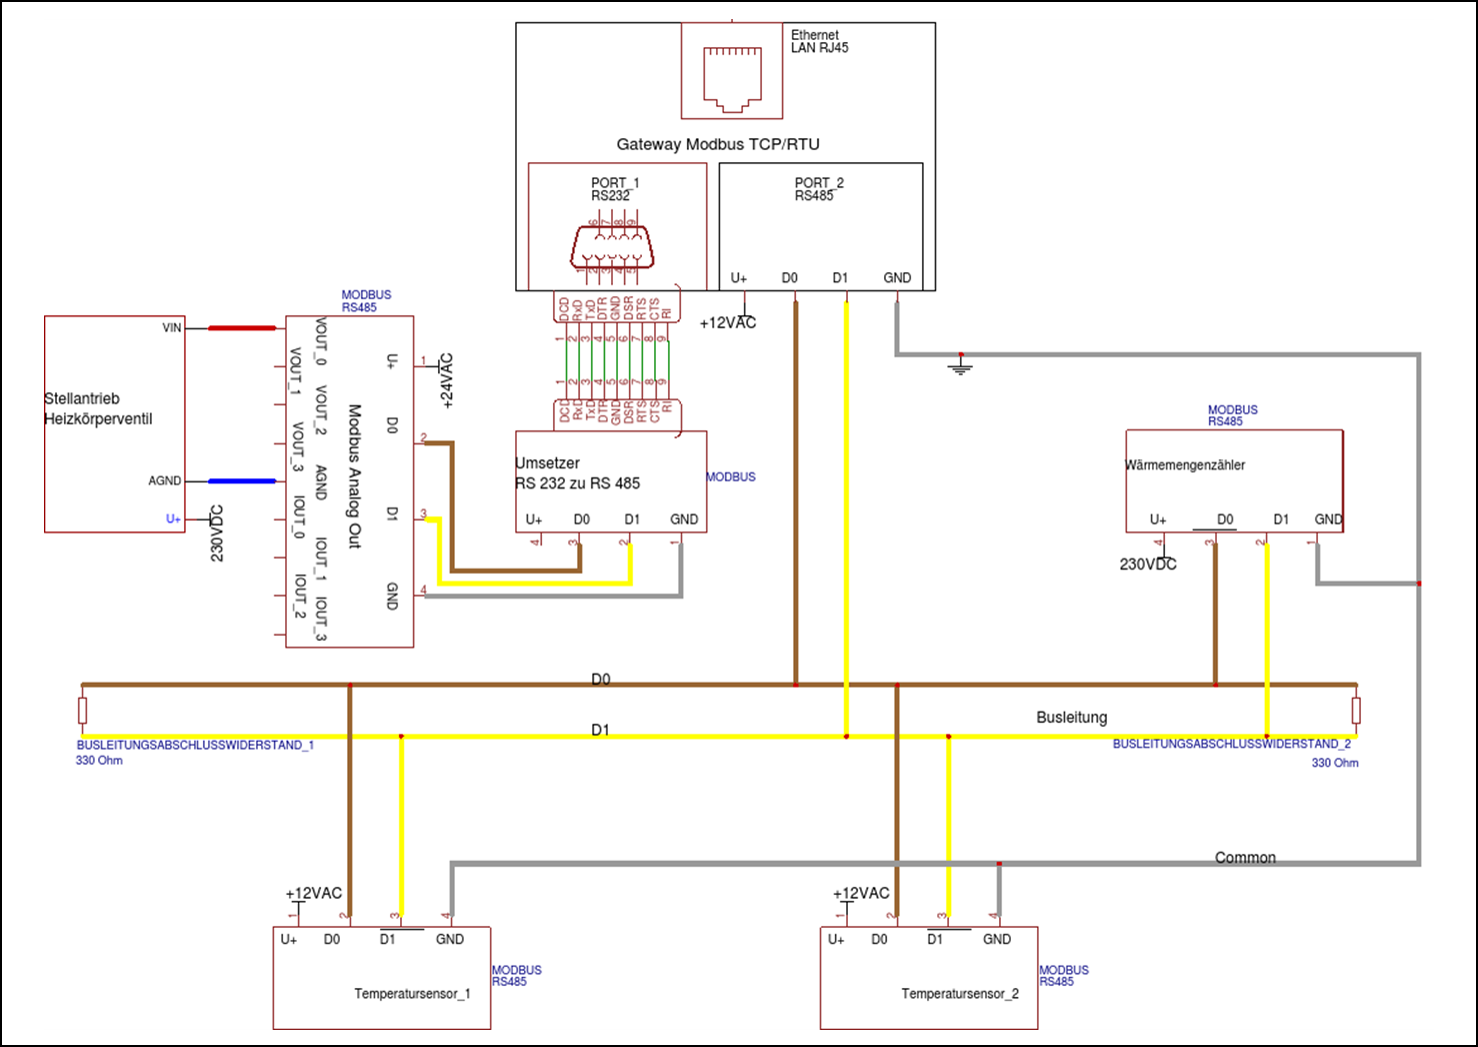
\includegraphics[width=\textwidth]{abbildungen/20160326_schaltplan}
\caption{Schaltplan der Raumtemperaturregelungsanlage}
\label{fig:schaltplan}
\end{figure}

Die Konfiguration des RS 485 Netzwerks geschieht über das Gateway und dessen Einstellungen sind in Tabelle \ref{tab:konfport} zusammengefasst.

\begin{table}[H]
\centering
\small
\renewcommand{\arraystretch}{1.3}
\begin{tabularx}{1\textwidth}{m{0.3\textwidth}m{0.3\textwidth}m{0.3\textwidth}}

\toprule

\textbf{Konfigurationsmerkmal} & \textbf{Werte Port 1} & \textbf{Werte Port 2} \\

\cmidrule[0.5pt](r{0.25em}){1-1} 
\cmidrule[0.5pt](l{0.25em}){2-2}
\cmidrule[0.5pt](l{0.25em}){3-3}

Port & 502\\

\ccol Baudrate & \ccol	19200 [$\frac{bits}{S}$]& \ccol	9600 [$\frac{bits}{S}$]	\\

Parität	& Gerade & Keine		\\

\ccol Datenbitlänge & \ccol 8 & \ccol 8	\\

Stoppbitlänge & 1 &	1	\\

\ccol Timeoutzeit &	\ccol 10 [$mS$] & \ccol 10 [$mS$]	\\

Betriebsweise 	&	Modbus TCP zu RTU\newline Server &	Modbus TCP zu RTU\newline Server \\


\bottomrule
\end{tabularx}
\caption{Netzwerkkonfiguration der Ports des EX9132M-MTCP Gatways}
\label{tab:konfport}
\end{table}


Bei der Inbetriebnahme der Anlage ergab sich jedoch eine Schwierigkeit bei der Kommunikation. Es hat sich herausgestellt, dass der Signalwandler EX9024M nicht streng nach den Modbus Spezifikationen für serielle Kommunikation hergestellt wird. Dadurch ergibt sich keine kompatible Netzwerkkonfiguration, um diesen zusammen mit den beiden Raumtemperaturfühlern in einem Netzwerk zu betreiben. Da das Gateway jedoch mit zwei Ports ausgestattet ist, konnte der zweite genutzt werden um ein weiteres serielles Netzwerk aufzubauen und damit das Problem zu lösen. Hierfür wurde ein Bridge in der Form eines einfachen Adapters eingesetzt, der die Spannungspegel und Steckerbelegungen des RS 232 Ports auf die einer RS 485 Schnittstelle umsetzt, wie im Schaltplan in \ref{fig:schaltplan} dargestellt.


\subsection{Software}

Um die zentral Steuerung vom Controller aus vorzunehmen, müssen die Schnittstellen der einzelnen Komponenten und deren Protokolle genutzt werden um alle von einer Python Konsole aus genutzt werden zu können. Wie bereits erwähnt bietet Python sehr viele Pakete die Funktionalitäten bereitstellen. Nichtsdestrotrotz muss eine eigene anlagenspezifische Software entwickelt werden, die diese Funktionalitäten jedoch nutzen kann. Der gesamte folgende Programmcode erfolgt objektorientiert und versucht eine klare Struktur und Wiederverwendbarkeit der einzelnen Methoden und Klassen zu gewährleisten. Das oberste Ziel der Programmierung ist es, eine einfache Bedienbarkeit der Anlage zu ermöglichen, also eine Bedienung ohne Kenntnisse über die zugrundeliegende Kommunikationstechnik zu ermöglichen.

Um die vier Temperatursensoren über den Webthermograph8x auszulesen wurde das Python Paket httlib genutzt. Die Abfrage der einzelnen Temperatursensoren über das HTTP Protokoll wurde in einer eigenen Klasse SensorsHttp implementiert und nutzt das HTTPConnection Objekt aus der httplib. Die konkrete Umsetzung der Klasse ist in Listing \ref{lst:webtemp} dargestellt.

Um die Verbindung zum Thermograph8x herzustellen wird dessen IP Adresse benötigt und die Port Nummer, über die die Telegramme gesendet und empfangen werden. Aus Gründen des Zugriffsschutzes sind diese Werte nicht im Code hinterlegt, sondern in den Umgebungsvariablen server-address und server-port der Pythonkonsole des Controllers.
Bei der Initialisierung wird mit der init-Methode ein HTTPConnection Objekt server erstellt, welches als Host und Port die Adressen des Webthermographen übergeben bekommt.
Des Weiteren wird jeweils eine Methode zur Herstellung und zur Trennung der Verbindung definiert sowie eine abstrakte Methode get-wt, welche die allgemeine Abfragesyntax der Messwerte enthält. Die Messwerte können lediglich einzeln abgefragt werden, über eine einfache Serveranfrage request, welche die Messwerte durch einen einfachen Befehls-string, \Gun GET\textbackslash Single \Gob zusammen mit der ID des gewünschten Temperatursensors, anfordert. Nachdem der Messwert in einen float Datentyp umgewandelt zurückgegeben wurde wird am Ende die Verbindung zum Server wieder getrennt. Die Methoden zum Auslesen der einzelnen Messwerte rufen lediglich die abstrakte Methode auf und übergeben dabei die ID des gewünschten Temperatursensors.

\lstinputlisting[language=Python ,caption={Klasse SensorsHttp zur Abfrage der Temperaturen vom Webthermograph8x}, label=lst:webtemp]{listings/sensors_http.py}

Für die Kommunikation mit den Modbus Komponenten stehen drei verschiedene Python Pakete zur Verfügung. Da Minimalmodbus leider keine Unterstützung für das Mobus TCP Protkoll bietet, kann es nicht zum Einsatz kommen. Nach ausführlicher Recherche über die beiden verbleibenden Pakete, fiel die Entscheidung pymodbus einzusetzen, da dessen Funktionsumfang viel umfangreicher und Dokumentation ausführlicher gestaltet und mit einfachen Beispielen gespickt ist.
Mit Hilfe der des pymodbus Pakets wurde daher zunächst wieder eine eigene Klasse ModbusConnection für die Kommunikation programmiert, welche in \ref{lst:modconnect} zu sehen ist.

Damit über das Modbus TCP Protokoll kommuniziert werden kann, muss auch hier zunächst eine Verbindung zwischen Client/Master und Server/Slave hergestellt werden. Für die Kommunikation wird das ModbusClient Objekt genutzt, da der Controller als Client über das Modbus TCP Protokol Anfargen an die Server stellt. Konkret stellt der Controller lediglich an das Gateway als Server Anfragen, welches die Telegramme in das serielle Modbus RTU Protokoll übersetzt um mit den Komponenten in den seriellen Netzwerken zu kommunizieren. Bei der Initialisierung werden wiederum die IP Adresse client-adress und der Port client-port benötigt über den die Kommunikation stattfindet. Des Weiteren wurden eigene Methoden zum Verbinden und Trennen implementiert, welche bei der Initilisierung genutzt werden. Eine Besonderheit stellt die delete-Methode dar, die im Falle eines Fehlers oder sterben einer Instanz der Klasse die Verbindung trennt. 
Zudem sind Methoden für die benötigten Zugriffe gemäß dem Modbus Datenmodell auf die Datentabellen implementiert. Diese umfassen das Auslesen von input- und holding-registers und liefern ein register zurück, was je nach Datenmodell einen Datentyp besitzt. Für die beiden Lesemethoden wird ein maximales probieren von 10 mal vorgesehen, bei einem Fehlversuch wird eine Pause von 1,5 sekunden gemacht bevor der nächste versuch gestartet wird. Für die Abfrage wird die Adresse in der Tabelle benötigt, die Anzahl der auszulesenden Worte/register/Datentypen sowie die Slave/Server-ID. Die letzte Methode um Register zu schreiben wird auf 3 Versuche begrenzt, ebenfalls mit Pause bei Fehler. Auch hier wird die Adresse in der Tabelle sowie die Slave/Server ID um den ebenfalls mitzugebenden Wert zu schreiben benötigt.
Damit sind die grundlegenden Funktionen für die Modbus Kommunikation implementiert und können zum Auslesen und Schreiben von Werten genutzt werden.

\lstinputlisting[language=Python ,caption={Klasse zum Verbindungsaufbau und Für die Grundfunktionen über Modbus TCP}, label=lst:modconnect]{listings/modbus_connection.py}

Diese Grundfunktionen werden von der SensorsModbus Klasse genutzt, um die Messwerte einzeln von den Sensoren abzufragen. Der Code dazu ist in Listing \ref{lst:modread} abgebildet.
Eine Besonderheit ist beim Auslesen der Werte aus dem Wärmemengenzähler gegeben, da dessen einzelne Messwerte die Größe eines Registers übersteigt. Wie in Abschnitt XXXXX bereits erwähnt, werden die Daten dann gemäß der Big-Endian Codierung verschlüsselt und müssen decodiert werden. Dazu bietet pymodbus ebenfalls eine entsprechende Funktion durch den BinaryPayload Decodierer mit der Besonderheit an, dass die Codierung little und big vertauscht sind bzw dass das gewünschte format angegeben werden muss. Die Länge von 2 Registern der Daten ist im Count angegeben und die ID im seriellen Netzwerk des Wärmemengenzählers ist ebenfalls angegeben. Die konkreten einzelnen Messwerte haben verschiedene Adressen in der Datentabelle welche in den Methoden gespeichert sind.
Die Adressen finden sich in Tabelle im Datenblatt im Anhang bzw in Tabelle.
Die beiden Temperatursensoren geben den Temperaturwert als integer ganzzahligen Wert zurück um eine Zehnerpotenz erhöht. Daher müssen auch dessen Werte decodiert werden durch eine Division durch zehn. Sie stehen jeweils in derselben Tabelle unter der gleichen Adresse, jedoch haben die beiden Temperatursensoren unterschiedliche IDs zugewiesen bekommen, durch die Schalterstellung gemäß Datenblatt/Adressmapping.

\lstinputlisting[language=Python ,caption={Klasse zum Auslesen über Modbus TCP}, label=lst:modread]{listings/sensors_modbus.py}

Die Klasse AcuatorsModbus erweitert ebenfalls die ModbusConnection Klasse, allerdings um die Aktuatoren anzusteuern. Dazu wird der Spannungsausgang am EX9024M mithilfe der dezimalen Registerwerten zwischen 8191 und 16383 gesteuert, die sich aus den Hexadezimalwerten im Datenblatt REFXXX ergeben. Der Maximalwert entspricht einer Ausgangsspannung von 10 V, der Minimalwert entsprechend 0 V. Im Rahmen der Anlagensteuerung soll jedoch nicht die Ausgangsspannung, sondern die Ventilstellung gesetzt werden. Um die Ventilstellung opening-level direkt anzugeben, 0 für Ventil zu und 1 für voll offen, erfolgt eine Umrechnung, zunächst in den entsprechenden Spannungswert und anschließend in den Registerwert der in die Datentabelle geschrieben wird. Außerdem wurde eine Methode zur Abfrage der Ventilstellung implementiert.

\lstinputlisting[language=Python ,caption={Klasse zum Auslesen über Modbus TCP}, label=lst:modact]{listings/actuators_modbus.py}

Um nun eine Bedienoberfläche zu schaffen die Plattformunabhängig bzw Kommunikationstechnologieunabhängig ist, wurden zwei weitere Klasse implementiert, die die jeweils vorausgegangenen Sensor und Aktor Klassen ein letztes Mal erweitert. Die Klassen Sensors und Actuators schaffen dies, indem sie die zuvor definierten Klassen importieren und bei der Initalisierung jeweils eine Instanz der Klasse bilden/instanzieren. Um die Unabhängigkeit von Kommunikationstechnologie zu erreichen, wird für jeden einzelnen Messwert eine eigene Methode mit eindeutiger Bezeichnung der Funktion und des Geräts definiert ohne dass ersichtlich ist welche Kommunikation darunter steckt. Damit ist ein Interface bze eine Oberfläche geschaffen die von Steuerungen genutzt werden können.

\lstinputlisting[language=Python ,caption={Die Actutators und Sensors Klassen zur Bedienung der Anlage}, label=lst:anlage]{listings/actuators.py}

\subsection{Inbetriebnahme mit Zweipunktregler}
Um die Funktion der Anlage zu überprüfen und bereits Messdaten zu sammeln, wurde ein erstes, einfaches Programm zur Regelung erstellt, welches bis zum Einsatz der Modellprädiktiven Regelung die Raumtemperaturregelugn übernimmt. Anhand dessen Programmablauf wird im Folgenden das Zusammenspiel der Anlage und die Ansteuerung der Anlagekomponenten erläutert.

Das Programm ist in Listing \ref{lst:oven} dargestellt und implementiert einen einfachen Zweipunktregler, der nach dem bekannten Backofenprinzip arbeitet und eine Schalthysterese von einem Grad Celsius besitzt. Zunächst werden die beiden Bedienoberflächen Sensors und Actuators importiert, gemeinsam mit einem Paket zum einfügen der Messwerte in eine Datenbank. Anschließend werden die verschiedenen Verbindungsparameter aus den Umgebungsvariablen der Pythonkonsole ausgelesen und zum Aufbau der Verbindung zu den Anlagenteilen und zur Datenbank genutzt. Dies geschieht durch die Instanzierung der Bedinoberflächeklassen Sensors und Actuators, die den Variablen s und a zugeiwesen werden.
 Des Weiteren werden die beiden Ventilstellungen für die Schaltpunkte definiert. Nun startet der eigentliche Steueralgorithmus innerhalb einer while-Schleife. Die dauerhafte Laufzeit wird über die Schleifenbedingung true erreicht, welche durch eine Tastenkombination oder bei Auftreten eines Fehlers gestoppt wird.
 Dabei werden die Verbindungen zu den Anlagenteilen trennt damit wird eine schnelle Wiederaufnahme des Betriebs gewährleistet wird und die Komponenten nicht durch eine bestehende Verbindung blockiert sind.
Zu Beginn werden alle Messwerte innerhalb der Anlage ausgelesen und das arithmetische Mittel der Raumtemperaturen einfach ermittelt. Die angenommene Raumtemperatur lässt sich über den Gewichtungsvektor weightings auch als gewichtetes arithmetisches Mittel berechnen.
Zum Auslesen der Werte, werden die Methoden des Sensors Objekts s und des Actuators Objekts a aufgerufen.
Das Abfangend von Fehlern wurde bereits in den unteren Klassen implementiert, sodass die Methoden zu Anlagenbedeinung einfach und robust sind. Außerdem wurden möglich eFehlebbdieungen ebenfalls ausgeschlossen an gegebenen Stellen, sodass z.B. unmögliche Ventilstellungen oder Werte nicht geschrieben oder angefordert werden können.

Anhand des Mittelwerts wird dann entschieden, ob der Heizkörper zur Raumerwärmung eingeschalten, weiter genutzt oder abgeschalten werden soll. Ist die Temperatur unter 21 Grad Celsius gestiegen und der Heizkörper wird noch nicht genutzt, erfolgt eine Ausgabe in der Konsole, dass es zu kalt ist und das Heizungsventil wird vollständig geöffnet. Ist die Temperatur über 22 Grad Celsius gestiegen und der Heizkörper wird genutzt, erfolgt eine Ausgabe, dass es zu warm ist, und das Heizungsventil wird geschlossen.
Danach erfolgt ein Update der Ventilstellung, bevor die Messdaten in der Konsole ausgegeben und in eine Datenbank eingefügt werden. Abschließend wartet die Steuerung für 60 Sekunden, bevor der Algorithmus von vorne beginnt/abläuft.

\lstinputlisting[language=Python ,caption={Zweipunktregler Programm zur Inbetriebnahme der Anlage}, label=lst:oven]{listings/oven_greedy_db.py}

Aus Gründen der Übersichtlichkeit sind die Abhängigkeiten zwischen den Klassen in Abbildung in einem UML Klassendiagramm in \ref{fig:uml} graphisch dargestellt. Eine llternative Modellprädiktive Regelung würde 

\begin{figure}
\centering
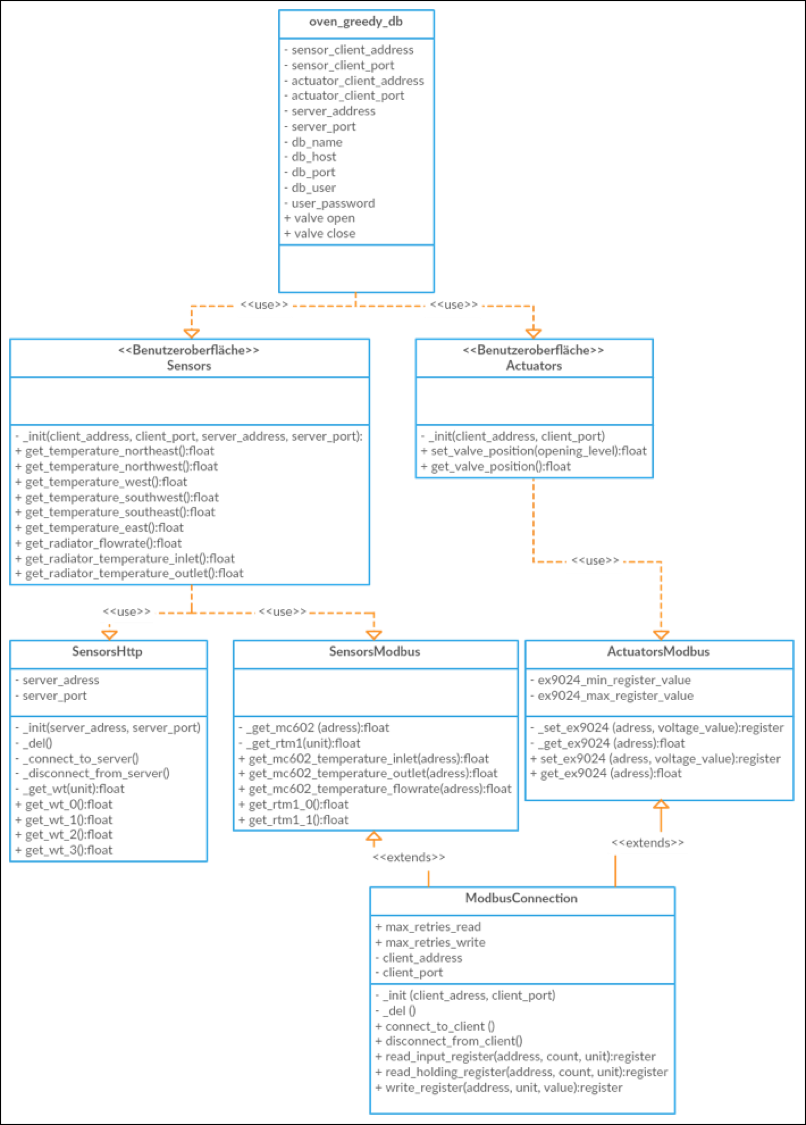
\includegraphics[width=\textwidth]{abbildungen/20160327_uml}
\caption{UML Klassendiagramm der zentralen Anlagensteuerung}
\label{fig:uml}
\end{figure}

Die Anlage konnte aufgrund von Lieferschwierigkeiten des Wärmemengenzählers erst am 16.12.2015 erfolgreich in Betrieb genommen werden. Seither siond lediglich kleinere Fehler aufgetreten, wodurch die Programmierung der Anlage stetig und sukszessive verbessert wurde.
Seit Mitte Januar läuft der Betrieb der Anlage durchgängig stabil und fehlerfrei und leistet einen sehr zuverlässigen Dienst.
Damit wird der Forderung nach einer hohen Funktionalität genüge getragen. Zudem wird auch die gewünschte Robustheit erfüllt, durch die fehlerabfangende Software.

Der gemessene Raumtemperaturverlauf über den Zeitraum von Mitte Januar bis Mitte April ist in REFXXXXX dargestellt und die These bestätigt werden, dass die Anlage eine Raumtemperatur regeln kann.
Aufgrund der zentralen Steuerung der Anlage, welche in Python umgesetzt wurde und fehlerfrei funktioniert, sind die Voraussetzungen für eine Regelbarkeit mit Hilfe von Modellprädiktiver Regelung erfüllt. Um die Eignung zu überprüfen, wird jedoch noch ein Modell des Raumes und der Anlage benötigt, welches im nachfolgenden Kapitel gebildet wird.